\chapter{\RU{Строки}\EN{Strings}}
\label{sec:digging_strings}

\section{\IFRU{Текстовые строки}{Text strings}}

\label{C_strings}
\IFRU{Обычные строки в Си заканчиваются нулем}{Usual C-strings are zero-terminated} 
(\ac{ASCIIZ}-\IFRU{строки}{strings}).

\IFRU{Причина, почему формат строки в Си именно такой (оканчивающийся нулем) вероятно историческая}
{The reason why C string format is as it is (zero-terminating) is apparently hisorical}.
\IFRU{В}{In} \cite{Ritchie79} \IFRU{мы можем прочитать}{we can read}:

\begin{framed}
\begin{quotation}
A minor difference was that the unit of I/O was the word, not the byte, because the PDP-7 was a word-addressed
machine. In practice this meant merely that all programs dealing with character streams ignored null
characters, because null was used to pad a file to an even number of characters.
\end{quotation}
\end{framed}

\index{Hiew}
\IFRU{Строки выглядят в Hiew или FAR Manager точно так же}{In Hiew or FAR Manager these strings looks like
as it is}:

\begin{lstlisting}
int main()
{
	printf ("Hello, world!\n");
};
\end{lstlisting}

\begin{figure}[H]
\centering
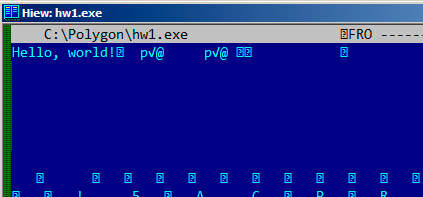
\includegraphics[scale=0.66]{digging_into_code/strings/C-string.png}
\caption{Hiew}
\end{figure}

\index{Pascal}
\index{Delphi}
\IFRU{Когда кодируются строки в Pascal и Delphi, сама строка предваряется 8-битным или 32-битным значением,
в котором закодирована длина строки}{The string is preceeded by 8-bit or 32-bit string length value}.

\IFRU{Например}{For example}:

\begin{lstlisting}[caption=Delphi]
CODE:00518AC8                 dd 19h
CODE:00518ACC aLoading___Plea db 'Loading... , please wait.',0

...

CODE:00518AFC                 dd 10h
CODE:00518B00 aPreparingRun__ db 'Preparing run...',0
\end{lstlisting}

\subsection{Unicode}

\index{Unicode}
\IFRU{Нередко уникодом называют все способы передачи символов, когда символ занимает 2 байта или 16 бит}
{Often, what is called by Unicode is a methods of strings encoding when each character occupies 2 bytes or 16 bits}.
\IFRU{Это распространенная терминологическая ошибка}{This is common terminological mistake}.
\IFRU{Уникод --- это стандарт, присваивающий номер каждому символу многих письменностей мира, но не описывающий
способ кодирования}{Unicode is a standard assigning a number to each character of many writing systems of the 
world, but not describing encoding method}.

\index{UTF-8}
\index{UTF-16LE}
\IFRU{Наиболее популярные способы кодирования}{Most popular encoding methods are}: 
UTF-8 (\IFRU{наиболее часто используется в Интернете и *NIX-системах}{often used in Internet and *NIX systems})
\AndENRU UTF-16LE (\IFRU{используется в}{used in} Windows).

\subsubsection{UTF-8}

\index{UTF-8}
UTF-8 \IFRU{это один из очень удачных способов кодирования символов}{is one of the most successful methods of
character encoding}.
\IFRU{Все символы латинницы кодируются так же, как и в ASCII-кодировке, а символы выходящие за пределы
ASCII-7-таблицы, кодируются несколькими байтами}{All Latin symbols are encoded just like in an ASCII-encoding,
and symbols beyond ASCII-table are encoded by several bytes}.
\IFRU{$0$ кодируется, как и прежде, нулевыми байтом, так что все стандартные
ф-ции Си продолжают работать с UTF-8-строками так же как и с обычными строками}{$0$ is encoded as it was
before, so all standard C string functions works with UTF-8-strings just like any other string}.

\IFRU{Посмотрим как символы из разных языков кодируются в UTF-8 и как это выглядит в FAR, в кодировке 437}
{Let's see how symbols in various languages are encoded in UTF-8 and how it looks like in FAR in 437 codepage}
\footnote{\IFRU{Я взял пример и переводы на разные языки здесь}{I've got example and translations from there}: 
\url{http://www.columbia.edu/~fdc/utf8/}}:

\begin{figure}[H]
\centering
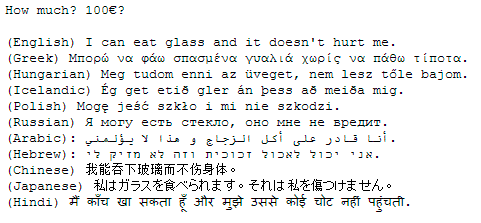
\includegraphics[scale=0.66]{digging_into_code/strings/multilang_sampler.png}
\end{figure}

\begin{figure}[H]
\centering
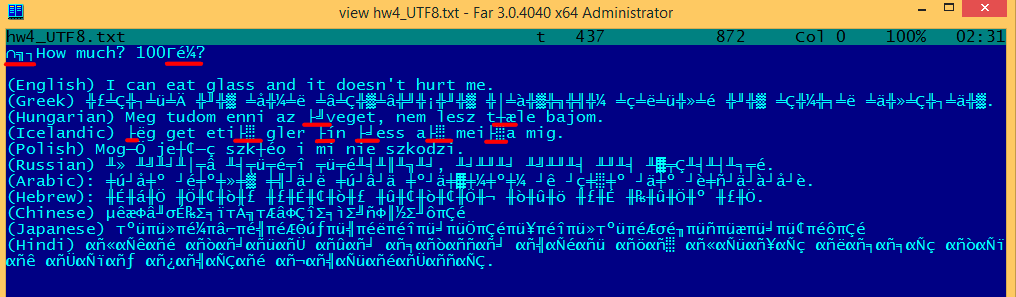
\includegraphics[scale=0.66]{digging_into_code/strings/multilang_sampler_UTF8.png}
\caption{FAR: UTF-8}
\end{figure}

\IFRU{Видно что строка на английском языке выглядит точно так же как и в ASCII-кодировке}
{As it seems, English language string looks like as it is in ASCII-encoding}.
\IFRU{В венгерском языке используются латинница плюс латинские буквы с диакритическими знаками}
{Hungarian language uses Latin symbols plus symbols with diacritic marks}.
\IFRU{Здесь видно что эти буквы кодируются несколькими байтами, я подчеркнул их красным}
{These symbols are encoded by several bytes, I underscored them by red}.
\IFRU{То же самое с исландским и польским языками}{The same story with Icelandic and Polish languages}.
\IFRU{В самом начале я также применил символ валюты ``Евро'', который кодируется тремя байтами}
{I also used ``Euro'' currency symbol at the begin, which is encoded by 3 bytes}.
\IFRU{Остальные системы письма здесь никак не связаны с латинницей}
{All the rest writing systems here have no connection with Latin}.
\IFRU{По крайней мере о русском, арабском, иврите и хинди мы можем сказать что здесь видны повторяющиеся
байты, что не удивительно, ведь, обычно буквы из одной и той же системы письменности расположены в одной
или нескольких таблицах уникода, поэтому часто их коды начинаются с одних и тех же цифр}
{At least about Russian, Arabic, Hebrew and Hindi we could see recurring bytes, and that is not surprise:
all symbols from the writing system is usually located in the same Unicode table, so their code begins with
the same numbers}.

\IFRU{В самом начале, перед строкой ``How much?'', видны три байта, которые на самом деле \ac{BOM}}
{At the very beginning, before ``How much?'' string we see 3 bytes, which is \ac{BOM} in fact}.
\ac{BOM} \IFRU{показывает, какой способ кодирования будет сейчас использоваться}{defines encoding system to be
used now}.

\subsubsection{UTF-16LE}

\index{UTF-16LE}
\index{Win32}
\IFRU{Многие ф-ции win32 в Windows имееют суффикс}{Many win32 functions in Windows has a suffix} \TT{-A} 
\AndENRU \TT{-W}.
\IFRU{Первые ф-ции работают с обычными строками, вторые с UTF-16LE-строками}{The first functions works
with usual strings, the next with UTF-16LE-strings} (\IT{wide}).
\IFRU{Во втором случае, каждый символ обычно хранится в 16-битной переменной типа \IT{short}}
{As in the second case, each symbol is usually stored in 16-bit value of \IT{short} type}.

\IFRU{Cтроки с латинскими буквами выглядят в Hiew или FAR как перемежающиеся с нулевыми байтами}
{Latin symbols in UTF-16 strings looks in Hiew or FAR as interleaved with zero byte}:

\begin{lstlisting}
int wmain()
{
	wprintf (L"Hello, world!\n");
};
\end{lstlisting}

\begin{figure}[H]
\centering
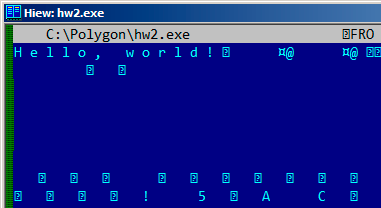
\includegraphics[scale=0.66]{digging_into_code/strings/UTF16-string.png}
\caption{Hiew}
\end{figure}

\IFRU{Подобное можно часто увидеть в системных файлах \gls{Windows NT}}{We may often see this in \gls{Windows NT} 
system files}:

\begin{figure}[H]
\centering
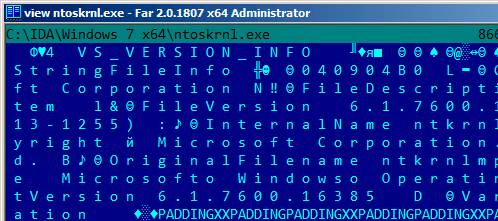
\includegraphics[scale=0.66]{digging_into_code/strings/ntoskrnl_UTF16.png}
\caption{Hiew}
\end{figure}

\index{IDA}
\IFRU{В \IDA, уникодом называется именно строки с символами занимающими 2 байта}{String with characters
occupying exactly 2 bytes are called by ``Unicode'' in \IDA}:

\begin{lstlisting}
.data:0040E000 aHelloWorld:
.data:0040E000                 unicode 0, <Hello, world!>
.data:0040E000                 dw 0Ah, 0
\end{lstlisting}

\IFRU{Вот как может выглядеть строка на русском языке}{Here is how Russian language 
string}\RU{ (``И снова здравствуйте!'')} \IFRU{закодированная в UTF-16LE}{encoded in UTF-16LE may looks like}:

\begin{figure}[H]
\centering
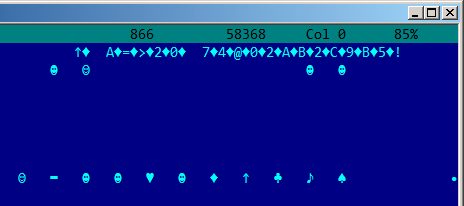
\includegraphics[scale=0.66]{digging_into_code/strings/russian_UTF16.png}
\caption{Hiew: UTF-16LE}
\end{figure}

\IFRU{То что бросается в глаза --- это то что символы перемежаются ромбиками (который имеет код 4)}
{What we can easily spot---is that symbols are interleaved by diamond character (which has code of 4)}.
\IFRU{Действительно, в уникоде кирилличные символы находятся в четвертом блоке}{Indeed, Cyrillic symbols
are located in the fourth Unicode plane}
\footnote{\url{https://en.wikipedia.org/wiki/Cyrillic_(Unicode_block)}}.
\IFRU{Таким образом, все кирилличные символы в UTF-16LE находятся в диапазоне}{Hence, all
Cyrillic symbols in UTF-16LE are located in} \TT{0x400-0x4FF}\EN{ range}.

\IFRU{Вернемся к примеру, где одна и та же строка написана разными языками}{Let's back to the example with the
string written in multiple languages}.
\IFRU{Здесь посмотрим в кодировке UTF-16LE}{Here we can see it in UTF-16LE encoding}.

\begin{figure}[H]
\centering
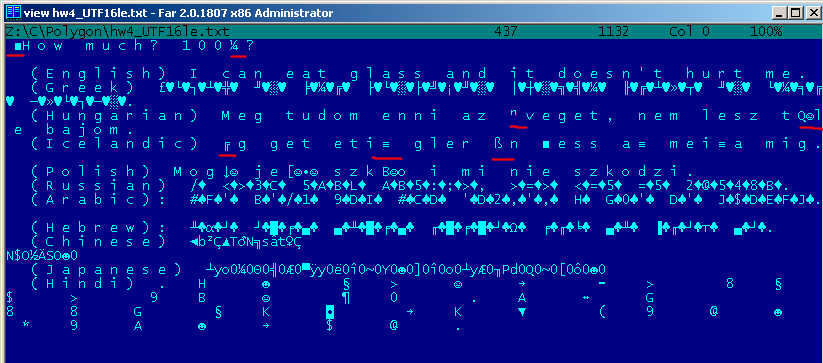
\includegraphics[scale=0.66]{digging_into_code/strings/multilang_sampler_UTF16.png}
\caption{FAR: UTF-16LE}
\end{figure}

\IFRU{Здесь мы так же видим \ac{BOM} в самом начале}{Here we can also see \ac{BOM} in the very beginning}.
\IFRU{Все латинские буквы перемежаются с нулевыми байтом}{All Latin characters are interleaved with zero byte}.
\IFRU{Некоторые буквы с диакритическими знаками (венгерский и исландский языки) также подчеркнуты красным}
{I also underscored by red some characters with diacritic marks (Hungarian and Icelandic languages)}.

% TODO: strings *NIX utility. procmonitor also shows strings...



\section{\RU{Сообщения об ошибках и отладочные сообщения}\EN{Error/debug messages}}

\RU{Очень сильно помогают отладочные сообщения, если они имеются. В некотором смысле, отладочные сообщения, 
это отчет о том, что сейчас происходит в программе.
Зачастую, это \printf-подобные функции, 
которые пишут куда-нибудь в лог, а бывает так что и не пишут ничего, но вызовы остались, так как эта сборка ~--- 
не отладочная, а \IT{release}.}
\EN{Debugging messages are very helpful if present.
In some sense, debugging messages are reporting
about what's going on in program right now. Often these are \printf-like functions,
which writes to log-files, and sometimes, not writing anything but calls are still present 
since this build is not a debug build but \IT{release} one.}
\index{\oracle}
\RU{Если в отладочных сообщениях дампятся значения некоторых локальных или глобальных переменных, 
это тоже может помочь, как минимум, узнать их имена. 
Например, в \oracle одна из таких функций: \TT{ksdwrt()}.}
\EN{If local or global variables are dumped in debugging messages, it might be helpful as well 
since it is possible to get variable names at least.
For example, one of such functions in \oracle is \TT{ksdwrt()}.}

\RU{Осмысленные текстовые строки вообще очень сильно могут помочь. 
Дизассемблер \IDA может сразу указать, из какой функции и из какого её места используется эта строка. 
Встречаются и смешные случаи}
\EN{Meaningful text strings are often helpful.
\IDA disassembler may show from which function and from which point this specific string is used.
Funny cases sometimes happen}\footnote{\href{http://go.yurichev.com/17223}{blog.yurichev.com}}.

\RU{Сообщения об ошибках также могут помочь найти то что нужно. 
В \oracle сигнализация об ошибках проходит при помощи вызова некоторой группы функций. \\
Тут еще немного об этом}
\EN{Error messages may help us as well.
In \oracle, errors are reporting using group of functions.\\
More about it}: \href{http://go.yurichev.com/17224}{blog.yurichev.com}.

\index{Error messages}
\RU{Можно довольно быстро найти, какие функции сообщают о каких ошибках, и при каких условиях.}
\EN{It is possible to find very quickly, which functions reporting about errors and in which conditions.}
\RU{Это, кстати, одна из причин, почему в защите софта от копирования, 
бывает так, что сообщение об ошибке заменяется 
невнятным кодом или номером ошибки. Мало кому приятно, если взломщик быстро поймет, 
из-за чего именно срабатывает защита от копирования, просто по сообщению об ошибке.}
\EN{By the way, it is often a reason why copy-protection systems has inarticulate cryptic error messages 
or just error numbers. No one happy when software cracker quickly understand why copy-protection
is triggered just by error message.}

\RU{Один из примеров шифрования сообщений об ошибке, здесь}\EN{One example of encrypted error messages 
is here}: \ref{examples_SCO}.

\section{\EN{Suspicious magic strings}\RU{Подозрительные магические строки}}

\EN{Some magic strings which are used in backdoors looks pretty suspicious.}
\RU{Некоторые магические строки, используемые в бэкдорах выглядят очень подозрительно.}
\RU{Например, в домашних роутерах TP-Link WR740 был бэкдор}
\EN{For example, there was a backdoor in TP-Link WR740 home router}\footnote{\url{http://sekurak.pl/tp-link-httptftp-backdoor/}\RU{, на русском: \url{http://m.habrahabr.ru/post/172799/}}}.
\RU{Бэкдор активировался при посещении следующего URL:}\EN{Backdoor was activated using the following URL:}\\
\url{http://192.168.0.1/userRpmNatDebugRpm26525557/start_art.html}.
\RU{Действительно, строка ``userRpmNatDebugRpm26525557'' присутствует в прошивке.}
\EN{Indeed, ``userRpmNatDebugRpm26525557'' string is present in firmware.}
\RU{Эту строку нельзя было нагуглить до распространения информации о бэкдоре.}
\EN{This string was not googleable upon wide backdoor information disclosure.}
\RU{Вы не найдете ничего такого ни в одном \ac{RFC}.}
\EN{You would not find this in any \ac{RFC}.}
\RU{Вы не найдете ни одного алгоритма в компьютерных науках, 
которые бы использовали такие странные последовательности байт.}
\EN{You would not find any computer science algorithm which may use such strange byte sequences.}
\RU{И это не выглядит как сообщение об ошибке, или отладочное сообщение.}
\EN{And it doesn't look like error or debugging message.}
\RU{Так что проверить использование подобных странных строк --- это всегда хорошая идея.}
\EN{So it's a good idea to inspect usage of such weird strings.}\\
\\
\index{base64}
\RU{Иногда такие строки кодируются при помощи}
\EN{Sometimes, such strings are encoded using}
base64\RU{\footnote{Например, бэкдор в кабельном модеме Arris: 
\url{http://www.securitylab.ru/analytics/461497.php}}}.
\RU{Так что неплохая идея их всех декодировать и затем просмотреть глазами, пусть даже бегло.}
\EN{So it's a good idea to decode them all and to scan them visually, even superficially.}\\
\\
\index{Security through obscurity}
\EN{More preciously, such method of hiding backdoors is called ``security through obscurity''.}
\RU{Более точно, такой метод сокрытия бэкдоров называется ``security through obscurity'' (безопасность через
запутанность).}
